\documentclass{standalone}
\usepackage{tikz}
\usetikzlibrary{patterns, positioning}


\begin{document}
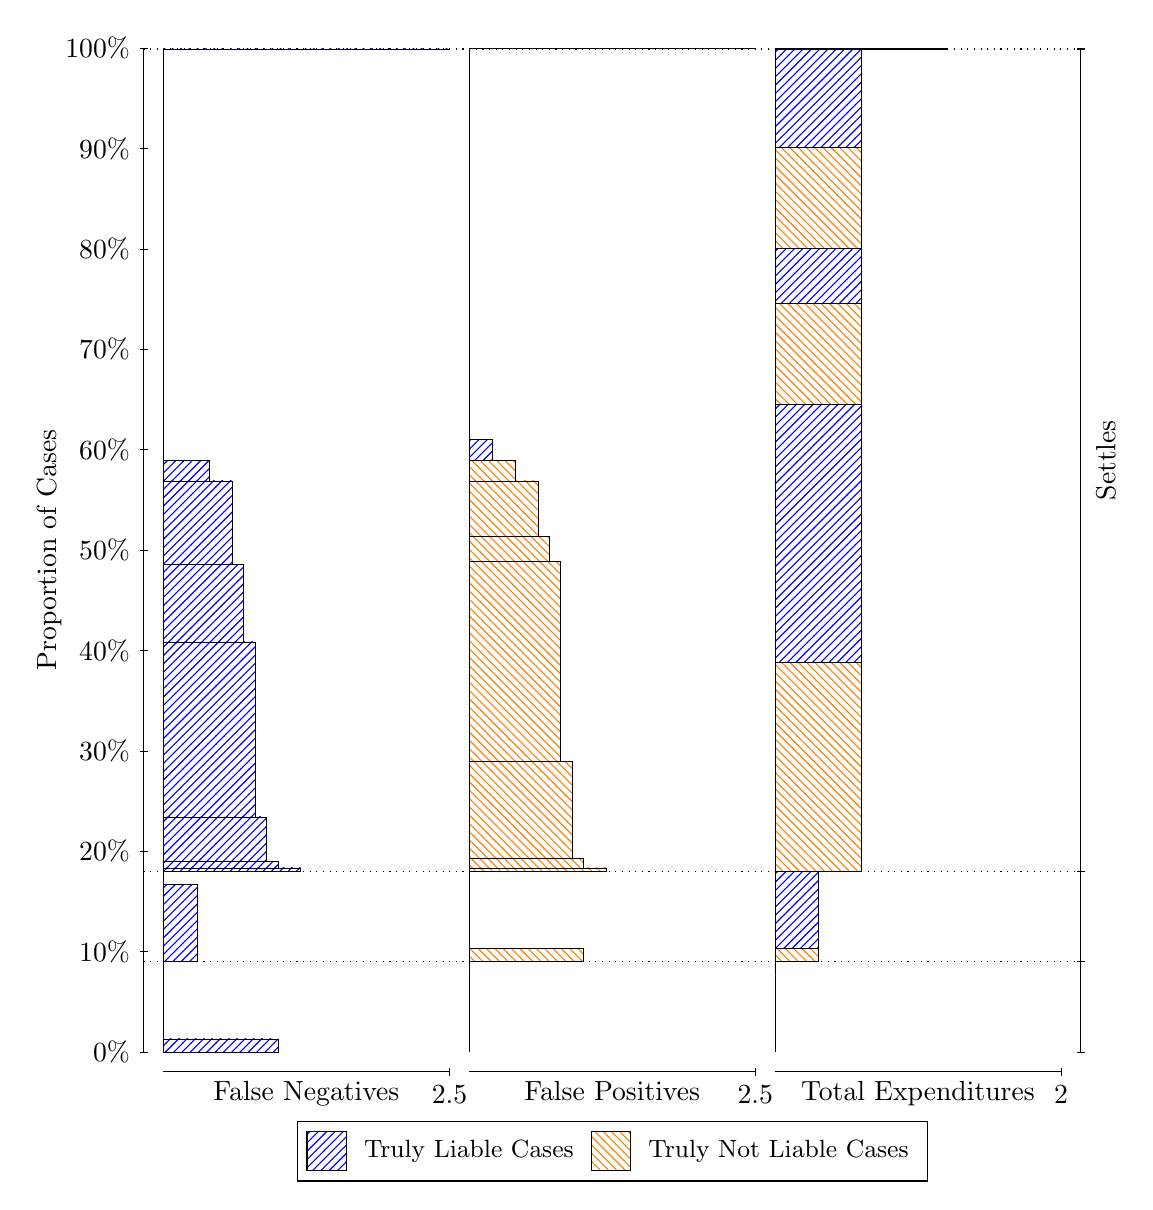
\begin{tikzpicture}
\draw[black, very thin] (1.5,1.75) -- (1.5,14.5);
\node[rotate=90, text=black, anchor=center] at (0.3, 8.125) {Proportion of Cases};
\draw[black, very thin] (1.45,1.75) -- (1.55,1.75);
\node[text=black, anchor=east] at (1.45, 1.75) {0\%};
\draw[black, very thin] (1.45,3.025) -- (1.55,3.025);
\node[text=black, anchor=east] at (1.45, 3.025) {10\%};
\draw[black, very thin] (1.45,4.3) -- (1.55,4.3);
\node[text=black, anchor=east] at (1.45, 4.3) {20\%};
\draw[black, very thin] (1.45,5.575) -- (1.55,5.575);
\node[text=black, anchor=east] at (1.45, 5.575) {30\%};
\draw[black, very thin] (1.45,6.85) -- (1.55,6.85);
\node[text=black, anchor=east] at (1.45, 6.85) {40\%};
\draw[black, very thin] (1.45,8.125) -- (1.55,8.125);
\node[text=black, anchor=east] at (1.45, 8.125) {50\%};
\draw[black, very thin] (1.45,9.4) -- (1.55,9.4);
\node[text=black, anchor=east] at (1.45, 9.4) {60\%};
\draw[black, very thin] (1.45,10.675) -- (1.55,10.675);
\node[text=black, anchor=east] at (1.45, 10.675) {70\%};
\draw[black, very thin] (1.45,11.95) -- (1.55,11.95);
\node[text=black, anchor=east] at (1.45, 11.95) {80\%};
\draw[black, very thin] (1.45,13.225) -- (1.55,13.225);
\node[text=black, anchor=east] at (1.45, 13.225) {90\%};
\draw[black, very thin] (1.45,14.5) -- (1.55,14.5);
\node[text=black, anchor=east] at (1.45, 14.5) {100\%};

\draw[black, very thin] (13.4,1.75) -- (13.4,14.5);
\draw[black, very thin] (13.35,1.75) -- (13.45,1.75);
\node[anchor=west] at (13.35, 1.75) {};
\draw[black, very thin] (13.35,2.8977) -- (13.45,2.8977);
\node[anchor=west] at (13.35, 2.8977) {};
\draw[black, very thin] (13.35,4.0423) -- (13.45,4.0423);
\node[anchor=west] at (13.35, 4.0423) {};
\draw[black, very thin] (13.35,14.487) -- (13.45,14.487);
\node[anchor=west] at (13.35, 14.487) {};
\draw[black, very thin] (13.35,14.493) -- (13.45,14.493);
\node[anchor=west] at (13.35, 14.493) {};
\draw[black, very thin] (13.35,14.5) -- (13.45,14.5);
\node[anchor=west] at (13.35, 14.5) {};

\draw[black, very thin, pattern color=blue, pattern=north east lines] (1.75,1.75) rectangle (3.2033,1.9156);
\draw[black, very thin, pattern color=orange, pattern=north west lines] (1.75,1.9156) rectangle (1.75,2.8977);
\draw[black, very thin, pattern color=blue, pattern=north east lines] (1.75,2.8977) rectangle (2.186,3.8782);
\draw[black, very thin, pattern color=orange, pattern=north west lines] (1.75,3.8782) rectangle (1.75,4.0423);
\draw[black, very thin, pattern color=blue, pattern=north east lines] (1.75,4.0423) rectangle (3.494,4.0868);
\draw[black, very thin, pattern color=blue, pattern=north east lines] (1.75,4.0868) rectangle (3.2033,4.1673);
\draw[black, very thin, pattern color=blue, pattern=north east lines] (1.75,4.1673) rectangle (3.058,4.7366);
\draw[black, very thin, pattern color=blue, pattern=north east lines] (1.75,4.7366) rectangle (2.9127,6.9582);
\draw[black, very thin, pattern color=blue, pattern=north east lines] (1.75,6.9582) rectangle (2.7673,7.945);
\draw[black, very thin, pattern color=blue, pattern=north east lines] (1.75,7.945) rectangle (2.622,9.0022);
\draw[black, very thin, pattern color=blue, pattern=north east lines] (1.75,9.0022) rectangle (2.3313,9.2644);
\draw[black, very thin, pattern color=orange, pattern=north west lines] (1.75,9.2644) rectangle (1.75,14.487);
\draw[black, very thin, pattern color=blue, pattern=north east lines] (1.75,14.487) rectangle (5.3833,14.489);
\draw[black, very thin, pattern color=orange, pattern=north west lines] (1.75,14.489) rectangle (1.75,14.493);
\draw[black, very thin, pattern color=orange, pattern=north west lines] (1.75,14.493) rectangle (1.75,14.496);
\draw[black, very thin, pattern color=blue, pattern=north east lines] (1.75,14.496) rectangle (1.75,14.5);
\draw[black, very thin, pattern color=orange, pattern=north west lines] (5.6333,1.75) rectangle (5.6333,2.7322);
\draw[black, very thin, pattern color=blue, pattern=north east lines] (5.6333,2.7322) rectangle (5.6333,2.8977);
\draw[black, very thin, pattern color=orange, pattern=north west lines] (5.6333,2.8977) rectangle (7.0867,3.0618);
\draw[black, very thin, pattern color=blue, pattern=north east lines] (5.6333,3.0618) rectangle (5.6333,4.0423);
\draw[black, very thin, pattern color=orange, pattern=north west lines] (5.6333,4.0423) rectangle (7.3773,4.0868);
\draw[black, very thin, pattern color=orange, pattern=north west lines] (5.6333,4.0868) rectangle (7.0867,4.2075);
\draw[black, very thin, pattern color=orange, pattern=north west lines] (5.6333,4.2075) rectangle (6.9413,5.4453);
\draw[black, very thin, pattern color=orange, pattern=north west lines] (5.6333,5.4453) rectangle (6.796,7.9792);
\draw[black, very thin, pattern color=orange, pattern=north west lines] (5.6333,7.9792) rectangle (6.6507,8.2973);
\draw[black, very thin, pattern color=orange, pattern=north west lines] (5.6333,8.2973) rectangle (6.5053,9.0022);
\draw[black, very thin, pattern color=orange, pattern=north west lines] (5.6333,9.0022) rectangle (6.2147,9.2644);
\draw[black, very thin, pattern color=blue, pattern=north east lines] (5.6333,9.2644) rectangle (5.924,9.5266);
\draw[black, very thin, pattern color=blue, pattern=north east lines] (5.6333,9.5266) rectangle (5.6333,14.487);
\draw[black, very thin, pattern color=orange, pattern=north west lines] (5.6333,14.487) rectangle (5.6333,14.491);
\draw[black, very thin, pattern color=blue, pattern=north east lines] (5.6333,14.491) rectangle (5.6333,14.493);
\draw[black, very thin, pattern color=orange, pattern=north west lines] (5.6333,14.493) rectangle (9.2667,14.496);
\draw[black, very thin, pattern color=blue, pattern=north east lines] (5.6333,14.496) rectangle (7.8133,14.5);
\draw[black, very thin, pattern color=orange, pattern=north west lines] (9.5167,1.75) rectangle (9.5167,2.7322);
\draw[black, very thin, pattern color=blue, pattern=north east lines] (9.5167,2.7322) rectangle (9.5167,2.8977);
\draw[black, very thin, pattern color=orange, pattern=north west lines] (9.5167,2.8977) rectangle (10.062,3.0618);
\draw[black, very thin, pattern color=blue, pattern=north east lines] (9.5167,3.0618) rectangle (10.062,4.0423);
\draw[black, very thin, pattern color=orange, pattern=north west lines] (9.5167,4.0423) rectangle (10.607,6.6968);
\draw[black, very thin, pattern color=blue, pattern=north east lines] (9.5167,6.6968) rectangle (10.607,9.9757);
\draw[black, very thin, pattern color=orange, pattern=north west lines] (9.5167,9.9757) rectangle (10.607,11.261);
\draw[black, very thin, pattern color=blue, pattern=north east lines] (9.5167,11.261) rectangle (10.607,11.955);
\draw[black, very thin, pattern color=orange, pattern=north west lines] (9.5167,11.955) rectangle (10.607,13.238);
\draw[black, very thin, pattern color=blue, pattern=north east lines] (9.5167,13.238) rectangle (10.607,14.487);
\draw[black, very thin, pattern color=orange, pattern=north west lines] (9.5167,14.487) rectangle (11.697,14.491);
\draw[black, very thin, pattern color=blue, pattern=north east lines] (9.5167,14.491) rectangle (11.697,14.493);
\draw[black, very thin, pattern color=orange, pattern=north west lines] (9.5167,14.493) rectangle (11.697,14.496);
\draw[black, very thin, pattern color=blue, pattern=north east lines] (9.5167,14.496) rectangle (11.697,14.5);
\draw[black, dotted] (1.5,2.8977) -- (13.4,2.8977);
\draw[black, dotted] (1.5,4.0423) -- (13.4,4.0423);
\draw[black, dotted] (1.5,14.487) -- (13.4,14.487);
\draw[black, dotted] (1.5,14.493) -- (13.4,14.493);
\draw[black, very thin] (1.75,1.5) -- (5.3833,1.5);
\node[text=black, anchor=north] at (3.5667, 1.5) {False Negatives};
\draw[black, very thin] (5.3833,1.45) -- (5.3833,1.55);
\node[text=black, anchor=north] at (5.3833, 1.45) {2.5};

\draw[black, very thin] (5.6333,1.5) -- (9.2667,1.5);
\node[text=black, anchor=north] at (7.45, 1.5) {False Positives};
\draw[black, very thin] (9.2667,1.45) -- (9.2667,1.55);
\node[text=black, anchor=north] at (9.2667, 1.45) {2.5};

\draw[black, very thin] (9.5167,1.5) -- (13.15,1.5);
\node[text=black, anchor=north] at (11.333, 1.5) {Total Expenditures};
\draw[black, very thin] (13.15,1.45) -- (13.15,1.55);
\node[text=black, anchor=north] at (13.15, 1.45) {2};



\node[text=black, centered, rotate=90] at (13.72, 9.2644) {Settles};



\draw (7.449999999999999,1.5) node[draw=none] (baseCoordinate) {};
\begin{scope}[align=center]
        \matrix[scale=0.5, draw=black, below=0.5cm of baseCoordinate, nodes={draw}, column sep=0.1cm]{
            \node[rectangle, draw, minimum width=0.5cm, minimum height=0.5cm, pattern color=blue, pattern=north east lines] {}; &
            \node[draw=none, font=\small, text=black] (B) {Truly Liable Cases}; &
            \node[rectangle, draw, minimum width=0.5cm, minimum height=0.5cm, pattern color=orange, pattern=north west lines] {}; &
            \node[draw=none, font=\small, text=black] (B) {Truly Not Liable Cases}; \\
            };
\end{scope}

\end{tikzpicture}
\end{document}